\documentclass[journal]{IEEEtran}

\usepackage{amsmath}
\usepackage{amssymb}
\usepackage{amsfonts}
\usepackage{amsthm}
\usepackage{mathtools}
\usepackage{bm}
\usepackage{algorithm}
\usepackage{algorithmic}
\usepackage{graphicx}
\usepackage{cite}
\usepackage{booktabs}
\usepackage{array}
\usepackage{url}

\renewcommand{\topfraction}{0.95}
\renewcommand{\textfraction}{0.05}

\newtheorem{theorem}{Theorem}
\newtheorem{lemma}{Lemma}
\newtheorem{corollary}{Corollary}
\newtheorem{definition}{Definition}
\newtheorem{assumption}{Assumption}
\newtheorem{remark}{Remark}

\newcommand{\R}{\mathbb{R}}
\newcommand{\E}{\mathbb{E}}
\newcommand{\Prob}{\mathbb{P}}
\newcommand{\KL}{D_{\mathrm{KL}}}
\newcommand{\relu}[1]{(#1)_{+}}

\begin{document}

\title{A Well-Posed, Uncertainty-Quantified Cell Digital Twin for In-Silico
Toxicology: Mechanistic Dynamics, Bayesian Calibration, and Online Data
Assimilation}

\author{Kunal~Achintya~Reddy~S%
\thanks{Source code, data, and the reproducible pipeline that generated every
figure and number in this article are openly available.}}

\markboth{}{}
\maketitle

\begin{abstract}
Predicting whether and how a compound harms a cell is central to toxicology and
drug safety, yet mechanistic models used for this purpose are typically closed,
report point estimates without calibrated uncertainty, and cannot be updated
online as new measurements arrive. This article presents a cell digital twin
that addresses these three gaps within a single, mathematically grounded, and
fully reproducible framework. The cell is represented as a five-state mechanistic
dynamical system---coupling mitochondrial energy, reactive oxygen species,
glutathione, an apoptotic commitment variable, and membrane integrity---driven
away from homeostasis by toxins that engage molecular targets through Hill
kinetics on a typed relation graph. We first prove that the governing dynamics
are well posed on the biologically admissible domain, with global existence,
uniqueness, and forward invariance, so the twin can never return a nonphysical
state. We then equip the model with Bayesian inference: a differentiable
re-implementation of the dynamics enables Hamiltonian Monte Carlo calibration
that yields half-maximal inhibitory concentrations (IC$_{50}$) with credible
intervals and an explicit identifiability diagnostic, and a gradient-free
particle filter assimilates streaming measurements so the twin's uncertainty
contracts as evidence accumulates. Calibrated against representative literature
cytotoxicity across an eighteen-toxin reference library, the model places
\emph{every} toxin with a standalone cytotoxic potency within one order of
magnitude (17/17) and reproduces their cross-compound potency ordering (Spearman
$\rho=0.996$; $\rho\approx0.88$ before any calibration, from mechanism alone). Across five cell types the twin
reproduces known tissue selectivity---anthracycline cardiotoxicity, cisplatin
nephro-selectivity, and tumor apoptosis-resistance---and metabolism-gated
toxicity. Parameter- and state-recovery experiments confirm the inference
machinery is correctly calibrated. The result is an open, uncertainty-aware
computational instrument for mechanism-aware toxicity screening.
\end{abstract}

\begin{IEEEkeywords}
Digital twin, quantitative systems toxicology, Bayesian inference, Hamiltonian
Monte Carlo, data assimilation, particle filter, uncertainty quantification,
dynamical systems, optimal experimental design.
\end{IEEEkeywords}

\section{Introduction}

\IEEEPARstart{Q}{uantitative} systems toxicology (QST) seeks to predict adverse
cellular outcomes from the molecular mechanisms that produce them, rather than
from empirical dose--response fitting alone \cite{bloomingdale2017,watkins2020}.
The dominant cellular injury axes---mitochondrial dysfunction, oxidative stress,
glutathione depletion, and the apoptotic/necrotic death decision---are shared
across a wide range of toxicants, which makes a compact mechanistic model of
these axes a natural substrate for screening \cite{yang2022,albeck2008}.
Mechanistic QST platforms such as DILIsym have demonstrated real regulatory value
along these lines \cite{watkins2020}. In parallel, the notion of a
\emph{digital twin}---a computational replica of a physical system that is
continuously reconciled with data---has moved from engineering into biomedicine
\cite{laubenbacher2022,corral2020}.

Three gaps limit the use of such models as decision instruments. First, most are
closed and not independently reproducible. Second, they report point predictions
without calibrated uncertainty, even though the underlying rate constants are
only known to within an order of magnitude and mechanistic ODE models are
notoriously ``sloppy''---many parameter combinations fit equally well
\cite{gutenkunst2007,transtrum2015}. Third, they are calibrated once and not
updated online, so they cannot function as a twin that tracks a specific
experimental preparation as measurements arrive.

This article develops a cell digital twin that closes these three gaps within one
framework, and does so in a way that is mathematically certified and openly
reproducible. Our contributions are:
\begin{enumerate}
\item A five-state mechanistic model of cellular injury, coupled to a typed
toxin--target relation graph through Hill kinetics, that we prove is globally
well posed on the biologically admissible domain (Theorem~\ref{thm:wellposed}):
the twin cannot silently produce a nonphysical state.
\item A Bayesian calibration layer built on a \emph{differentiable}
re-implementation of the dynamics, so Hamiltonian Monte Carlo (HMC) takes exact
gradients through the ODE and returns IC$_{50}$ posteriors with credible
intervals and an identifiability diagnostic. We recall the exactness of the
sequential update (Theorem~\ref{thm:filter}) and the parametric contraction rate
(Theorem~\ref{thm:contraction}) that justify it.
\item An online data-assimilation scheme (a particle filter) that infers an
unknown exposure and latent state from streaming measurements, with the credible
band contracting as evidence accumulates.
\item An empirical validation against representative literature cytotoxicity for
eighteen reference toxins across five cell types, demonstrating within-one-log
agreement, correct potency ordering, and reproduction of known tissue
selectivity and metabolism-gated toxicity.
\item An information-theoretic account of adaptive experiment selection
(Theorems~\ref{thm:eig}--\ref{thm:reduction}) that positions the twin for
economical, uncertainty-driven screening.
\end{enumerate}
The theoretical results we invoke are, individually, classical; the contribution
is their instantiation in, and empirical validation on, a concrete open cell
twin. Section~\ref{sec:model} presents the model and proves well-posedness;
Section~\ref{sec:inference} develops Bayesian calibration; Section~\ref{sec:design}
treats adaptive design; Section~\ref{sec:twin} defines the twin and its
assimilation; Section~\ref{sec:results} reports the empirical validation; and
Sections~\ref{sec:discussion}--\ref{sec:conclusion} discuss limitations and
conclude.

\section{The Governing Dynamical Model}
\label{sec:model}

\subsection{State, Domain, and Dynamics}

Let $\mathrm{ATP}(t)$, $\mathrm{ROS}(t)$, $\mathrm{GSH}(t)$ denote the normalized
mitochondrial energy charge, reactive-oxygen-species level, and glutathione
antioxidant pool; let $\mathrm{CASP}(t)\in[0,1]$ be the caspase/apoptotic
commitment and $\mathrm{MEM}(t)\in[0,1]$ the plasma-membrane integrity. Collect
$z=(\mathrm{ATP},\mathrm{ROS},\mathrm{GSH},\mathrm{CASP},\mathrm{MEM})^{\top}$ on
the biologically admissible domain
\[
\mathcal{D}=\{z\in\R^5: \mathrm{ATP},\mathrm{ROS},\mathrm{GSH}\ge0,\ \mathrm{CASP},\mathrm{MEM}\in[0,1]\}.
\]
A toxin exposure enters the dynamics only through a vector of dimensionless
\emph{process modifiers}
$m=(e,\,a,\,r,\,g,\,x,\,\mu,\,\alpha,\,\delta)$ derived below; with $\relu{\cdot}=\max(\cdot,0)$,
\begin{align}
\dot{\mathrm{ATP}} &= k_1\,e\,a - k_2\,\mathrm{ATP}, \label{eq:atp}\\
\dot{\mathrm{ROS}} &= b_0 + b_1(1-e) + b_2\,r - (s_0 + s_1\,\mathrm{GSH})\,\mathrm{ROS}, \label{eq:ros}\\
\dot{\mathrm{GSH}} &= q\,g - q_d\,\mathrm{GSH} - q_o\,\mathrm{ROS}\,\mathrm{GSH} - q_x\,x\,\mathrm{GSH}, \label{eq:gsh}\\
\dot{\mathrm{CASP}} &= c_1 T\,(1-\mathrm{CASP}) + c_2 \mathrm{CASP}(1-\mathrm{CASP}) - c_3 \mathrm{CASP}, \label{eq:casp}\\
\dot{\mathrm{MEM}} &= \rho\,(1-\mathrm{MEM}) - D\,\mathrm{MEM}, \label{eq:mem}
\end{align}
with apoptotic trigger and membrane-damage terms
\begin{align}
T &= w_r\relu{\mathrm{ROS}-\tau_r} + w_a\relu{\tau_a-\mathrm{ATP}} + w_\alpha\alpha + w_\delta\delta, \label{eq:trigger}\\
D &= d_\ell\,\mathrm{ROS}\,\relu{1-\mathrm{GSH}} + d_\mu\,\mu + d_n\relu{\tau_n-\mathrm{ATP}}. \label{eq:damage}
\end{align}
All rate constants are positive and are collected in $\theta$; their nominal
values (Table~\ref{tab:params}) are chosen so the unperturbed cell rests at the
homeostatic fixed point $z^\dagger=(1,\,\bar r,\,1,\,0,\,1)$ with
$\bar r = b_0/(s_0+s_1)$. The cell viability readout is $\Phi(z)=\mathrm{MEM}(1-\mathrm{CASP})$.
The crucial GSH-independent scavenging term $s_0>0$ in \eqref{eq:ros} represents
catalase/thioredoxin antioxidant capacity and, as shown below, is exactly what
bounds ROS when glutathione is exhausted.

\subsection{Toxin--Target Coupling on a Relation Graph}

The cell is annotated by a typed relation graph whose nodes (genes, proteins,
metabolites, organelles, phenotypes) map to the coupling processes above. A toxin
is a set of targets; target $j$ engages its node with fractional occupancy given
by the Hill function
\begin{equation}
o_j(\text{dose}) = \gamma\, e_j^{\max}\,\frac{\text{dose}^{\,h_j}}{\kappa_j^{h_j}+\text{dose}^{\,h_j}}, \label{eq:hill}
\end{equation}
where $\kappa_j$ is the target potency, $h_j$ the Hill coefficient, $e_j^{\max}\in(0,1]$
the maximal engagement, and $\gamma\in[0,1]$ a cytochrome-P450 bioactivation gate
(so metabolism-dependent toxins act only where $\gamma>0$). Occupancies aggregate
into the modifiers of \eqref{eq:atp}--\eqref{eq:damage}: multiplicatively for
inhibitory processes ($e=\prod(1-o_j)$ over electron-transport targets, similarly
$a,g$) and additively for generative processes ($r,x,\mu,\alpha,\delta=\sum o_j$).
Writing \eqref{eq:atp}--\eqref{eq:damage} compactly as
$\dot z=F(z,m(\text{dose};\theta);\theta)$, $z(0)=z_0\in\mathcal{D}$, gives the
object studied below.

\begin{table}[!t]
\renewcommand{\arraystretch}{1.1}
\caption{Nominal rate constants (homeostasis-preserving; see text)}
\label{tab:params}
\centering
\footnotesize
\begin{tabular}{@{}llll@{}}
\toprule
Sym. & Value & Sym. & Value \\
\midrule
$k_1,k_2$ (ATP prod./use) & $1.0,\,1.0$ & $c_1,c_2,c_3$ (caspase) & $0.5,\,0.3,\,0.05$\\
$b_0,b_1,b_2$ (ROS in) & $0.1,\,1.0,\,1.5$ & $\tau_r,\tau_a$ (thresholds) & $0.30,\,0.40$\\
$s_0,s_1$ (ROS scav.) & $0.5,\,1.5$ & $w_r,w_a$ & $1.0,\,1.0$\\
$q,q_d$ (GSH syn./turn.) & $0.55,\,0.50$ & $w_\alpha,w_\delta$ & $1.5,\,0.8$\\
$q_o,q_x$ (GSH consum.) & $1.0,\,1.0$ & $d_\ell,d_\mu,d_n$ (memb.) & $1.0,\,2.0,\,1.0$\\
$\rho$ (membrane repair) & $0.20$ & $\tau_n$ (necrosis thr.) & $0.20$\\
\bottomrule
\end{tabular}
\end{table}

\subsection{Well-Posedness}

\begin{theorem}[Existence, Uniqueness, Invariance]
\label{thm:wellposed}
For every $z_0\in\mathcal{D}$, every $\theta$ with strictly positive entries, and
every admissible exposure (any fixed dose in \eqref{eq:hill}, or any bounded
measurable dosing schedule), the initial value problem $\dot z=F(z,m;\theta)$,
$z(0)=z_0$ has a unique solution defined for all $t\ge0$, and $z(t)\in\mathcal{D}$
for all $t\ge0$.
\end{theorem}

\begin{proof}
\emph{Local existence and uniqueness.} $F$ is a sum of polynomial terms and the
Lipschitz maps $\relu{\cdot}$ in \eqref{eq:trigger}--\eqref{eq:damage}; hence $F$
is locally Lipschitz in $z$, uniformly on bounded sets. Picard--Lindel\"of gives
a unique solution on a maximal interval $[0,T_{\max})$.

\emph{Forward invariance.} By Nagumo's theorem \cite{blanchini1999}, a closed set
is invariant under a locally Lipschitz field provided $F$ is sub-tangential at
each boundary face. Evaluating $F$ on the faces of $\mathcal{D}$, using that the
remaining coordinates are admissible and every rate constant and modifier is
nonnegative:
\begin{align*}
\mathrm{ATP}{=}0:&\ \dot{\mathrm{ATP}}=k_1 e a\ge0; &
\mathrm{ROS}{=}0:&\ \dot{\mathrm{ROS}}=b_0+b_1(1{-}e)+b_2 r\ge0;\\
\mathrm{GSH}{=}0:&\ \dot{\mathrm{GSH}}=q g\ge0; &
\mathrm{CASP}{=}0:&\ \dot{\mathrm{CASP}}=c_1 T\ge0;\\
\mathrm{CASP}{=}1:&\ \dot{\mathrm{CASP}}=-c_3\le0; &
\mathrm{MEM}{=}0:&\ \dot{\mathrm{MEM}}=\rho\ge0;\\
\mathrm{MEM}{=}1:&\ \dot{\mathrm{MEM}}=-D\le0. &&
\end{align*}
In every case $F$ points into $\mathcal{D}$ or is tangent to it, so $\mathcal{D}$
is forward invariant.

\emph{Global existence.} It remains to exclude finite-time blow-up. From
\eqref{eq:atp}, $\dot{\mathrm{ATP}}\le k_1 - k_2\mathrm{ATP}$ (as $e,a\le1$), so
$\mathrm{ATP}(t)\le\max(\mathrm{ATP}(0),k_1/k_2)$. From \eqref{eq:gsh},
$\dot{\mathrm{GSH}}\le q - q_d\mathrm{GSH}$, so GSH is likewise bounded. The key
step is ROS: since $\mathrm{GSH}\ge0$, the scavenging coefficient satisfies
$s_0+s_1\mathrm{GSH}\ge s_0>0$, hence from \eqref{eq:ros}
\[
\dot{\mathrm{ROS}}\le \big(b_0+b_1+b_2\,r_{\max}\big) - s_0\,\mathrm{ROS},
\]
where $r_{\max}$ is the (bounded) maximal ROS input, so ROS is bounded by
Gr\"onwall's inequality \emph{even when glutathione is fully depleted}---this is
precisely the role of the GSH-independent term $s_0$. Finally
$\mathrm{CASP},\mathrm{MEM}\in[0,1]$ by invariance. The trajectory thus remains in
a compact subset of $\mathcal{D}$ on every finite interval, so the continuation
criterion \cite{khalil2002} gives $T_{\max}=\infty$.
\end{proof}

\begin{remark}
Theorem~\ref{thm:wellposed} is the prerequisite for using the model as a twin: it
certifies that for \emph{every} parameter draw from a posterior and \emph{every}
exposure, forward simulation returns a state in $\mathcal{D}$. Consequently the
predictive bands in Section~\ref{sec:results} never leave the admissible ranges,
which an uncertified system cannot guarantee.
\end{remark}

\section{Bayesian Calibration over the State Space}
\label{sec:inference}

\subsection{Observation Model and Differentiable Forward Map}

Measurements arrive at times $t_1<t_2<\cdots$ as
$y_k=h(z(t_k;\theta))+\varepsilon_k$, $\varepsilon_k\sim\mathcal{N}(0,\Sigma_k)$
independent across $k$, with $h$ a known observation map (e.g., an endpoint
viability assay, or a time course of ATP and ROS reporters). To make the
posterior tractable at scale, the dynamics \eqref{eq:atp}--\eqref{eq:damage} are
re-implemented as a fixed-step differentiable integrator, so gradients of the
likelihood with respect to $\theta$ propagate through the ODE and enable
gradient-based Hamiltonian Monte Carlo; the differentiable map is verified to
match a stiff reference solver to within $2\times10^{-2}$ in viability across all
toxins (Section~\ref{sec:results}).

\begin{theorem}[Exactness of Sequential Updating]
\label{thm:filter}
Let $p(\theta)$ be a prior and $p(y_k\mid\theta)$ the likelihood induced by
\eqref{eq:atp}--\eqref{eq:damage} through $h$. Define $p_0=p$ and
$p_k(\theta)\propto p(y_k\mid\theta)\,p_{k-1}(\theta)$. Then
$p_k(\theta)=p(\theta\mid y_{1:k})$ for every $k$.
\end{theorem}
\begin{proof}
By induction. The base case is the prior. Since $\theta$ is static and
$\varepsilon_k$ is independent across $k$, $y_k$ is conditionally independent of
$y_{1:k-1}$ given $\theta$, so $p(y_k\mid\theta,y_{1:k-1})=p(y_k\mid\theta)$.
Bayes' rule conditioned on $y_{1:k-1}$ with the inductive hypothesis
$p_{k-1}=p(\theta\mid y_{1:k-1})$ yields the stated recursion \cite{sarkka2013}.
\end{proof}

\subsection{Posterior Contraction}

\begin{assumption}[Identifiability]
\label{ass:ident}
$\ell(\theta)=\log p(y_k\mid\theta)$ is $C^2$ near the true (best-fitting)
$\theta^\star$, and the per-observation Fisher information
$I(\theta^\star)=-\E_{\theta^\star}[\partial^2_\theta\ell]$ is finite and positive
definite \cite{rao1945}.
\end{assumption}

\begin{theorem}[Parametric Contraction Rate]
\label{thm:contraction}
Under Assumption~\ref{ass:ident} with a prior continuous and positive at
$\theta^\star$ and $n$ conditionally independent observations,
$\sqrt n(\theta-\hat\theta_n)\mid y_{1:n}\xrightarrow{d}\mathcal{N}(0,I(\theta^\star)^{-1})$
in $\Prob_{\theta^\star}$-probability, where $\hat\theta_n$ is the MLE; hence the
posterior contracts around $\theta^\star$ in total variation at rate $O(n^{-1/2})$.
\end{theorem}
\begin{proof}
This is the Bernstein--von Mises theorem \cite{vandervaart1998}. A second-order
Taylor expansion of $\ell_n=\sum_k\log p(y_k\mid\theta)$ about $\hat\theta_n$ with
observed information $J_n=-\nabla^2\ell_n(\hat\theta_n)$, together with
$J_n/n\to I(\theta^\star)$ and $p(\theta)=p(\hat\theta_n)(1+o(1))$ on shrinking
neighborhoods, gives the Laplace approximation
$p_n(\theta)\approx\mathcal{N}(\theta;\hat\theta_n,J_n^{-1})$ with total-variation
error vanishing in probability; consistency of $\hat\theta_n$ and rescaling by
$\sqrt n$ give the stated limit and the $O(n^{-1/2})$ radius.
\end{proof}

\begin{remark}
Because ODE models are frequently sloppy \cite{gutenkunst2007}, Assumption
\ref{ass:ident} can fail along stiff parameter directions, and there the
posterior returns the prior rather than contracting. We do not hide this: we
report a per-parameter \emph{identifiability shrinkage}
$1-\mathrm{sd}_{\text{post}}/\mathrm{sd}_{\text{prior}}$, so prior-dominated
directions are disclosed (Section~\ref{sec:results}).
\end{remark}

\section{Adaptive Experimental Design}
\label{sec:design}

Let a design $d\in\mathcal{U}$ (e.g., a dose and measurement time) yield outcome
$Y_d$, and let $p(\theta)$ be the current posterior. The expected information gain
is $\mathrm{EIG}(d)=H[p(\theta)]-\E_{Y_d}\!\big[H[p(\theta\mid Y_d,d)]\big]$, with
$H$ the differential entropy \cite{cover2006,lindley1956}.

\begin{theorem}[EIG Identity and Nonnegativity]
\label{thm:eig}
For every $d\in\mathcal{U}$,
$\mathrm{EIG}(d)=I(\theta;Y_d)=\E_{Y_d}\big[\KL(p(\theta\mid Y_d,d)\,\|\,p(\theta))\big]\ge0$,
and if $\mathcal{U}$ is compact and $\mathrm{EIG}$ continuous then a maximizer
$d^\star$ exists and minimizes the expected posterior entropy.
\end{theorem}
\begin{proof}
The first equality is the entropy definition of mutual information; the second
follows by expanding the joint entropy in the opposite order and applying Bayes'
rule; nonnegativity is Gibbs' inequality $\KL(q\|r)\ge0$; existence follows from
the extreme value theorem \cite{chaloner1995}.
\end{proof}

\begin{theorem}[Sample Complexity and Reduction]
\label{thm:reduction}
Let $I(d)$ be the per-experiment Fisher information under design $d$. Under
Assumption~\ref{ass:ident} and Theorem~\ref{thm:contraction}, the number of
independent experiments to reach $\mathrm{tr}(\Sigma_n)\le\varepsilon$ is, to
leading order, $n(d)=\lceil\mathrm{tr}(I(d)^{-1})/\varepsilon\rceil$. If
$d^\star=\arg\max_{\mathcal U}\det I(d)$ dominates every $d$ in the Loewner order,
$I(d)\preceq I(d^\star)$, then $n(d^\star)\le n(d)$ for all $d\in\mathcal U$.
\end{theorem}
\begin{proof}
Additivity of Fisher information gives $\Sigma_n\approx I(d)^{-1}/n$, hence
$n(d)=\lceil\mathrm{tr}(I(d)^{-1})/\varepsilon\rceil$. Matrix inversion reverses
the Loewner order on the positive-definite cone: if $B\succeq A\succ0$ then
$A^{-1}\succeq B^{-1}$, and the trace is Loewner-monotone, so
$\mathrm{tr}(I(d)^{-1})\ge\mathrm{tr}(I(d^\star)^{-1})$ \cite{bhatia1997}.
\end{proof}

These results make adaptive, information-optimal screening well defined: the twin
evaluates $p(y\mid d)$ for candidate designs \emph{in silico} to choose the most
informative next experiment, a myopic surrogate that under the Laplace
approximation coincides with classical D-optimality.

\section{Digital Twin and Online Assimilation}
\label{sec:twin}

The digital twin of a preparation is the pair consisting of the posterior mean
trajectory $\bar z(t)=\E[z(t;\theta)\mid y_{1:k}]$ under the current posterior and
the posterior predictive covariance propagated through
\eqref{eq:atp}--\eqref{eq:damage}. Theorem~\ref{thm:wellposed} guarantees every
sampled trajectory stays in $\mathcal{D}$; Theorem~\ref{thm:filter} guarantees the
belief updates correctly; Theorem~\ref{thm:contraction} guarantees its
uncertainty shrinks with informative data.

For \emph{streaming} measurements the twin is updated by a bootstrap particle
filter \cite{gordon1993,doucet2001}: $N$ particles carry a latent state and an
unknown exposure parameter, are propagated through \eqref{eq:atp}--\eqref{eq:damage}
between observation times, weighted by the measurement likelihood, and resampled.
This is gradient-free and runs on the reference solver, complementing the
gradient-based HMC used for static calibration.

\section{Empirical Validation}
\label{sec:results}

All results below are produced by the open pipeline from the mechanistic engine;
each figure and number is regenerated by a single script.

\subsection{Calibration Against Literature Cytotoxicity}

We assembled representative literature cytotoxic IC$_{50}$ values for eighteen
reference toxins spanning mitochondrial inhibition (rotenone, antimycin~A,
cyanide, oligomycin, FCCP), oxidative stress (H$_2$O$_2$, menadione, paraquat,
tert-butyl hydroperoxide, arsenite), glutathione depletion (buthionine
sulfoximine), membrane disruption (Triton~X-100), direct apoptosis
(staurosporine), genotoxicity (etoposide, cisplatin, doxorubicin), and
CYP-bioactivated hepatotoxicity (acetaminophen, carbon tetrachloride).
Buthionine sulfoximine is a sensitizer with no standalone cytotoxic IC$_{50}$ and
is validated separately through synergy, leaving seventeen toxins with a
calibratable potency. Because a
toxin's effective cellular potency differs from its biochemical binding constant,
we calibrate a single scalar potency per toxin; the shape of every dose--response
curve and the cross-toxin ordering remain emergent model properties.

Fig.~\ref{fig:calibration} compares the model's emergent cytotoxic IC$_{50}$ to
the literature anchor for each toxin. After calibration \textbf{all 17/17 toxins} fall within one order of magnitude (median
fold-error 1.00$\times$), and the cross-toxin rank order matches with
Spearman $\rho=0.996$. Notably, \emph{before} any calibration the rank
correlation is already $\rho\approx0.88$: the mechanism orders compound potencies
essentially on its own, and calibration only fixes the absolute scale.

\begin{figure}[!t]
\centering
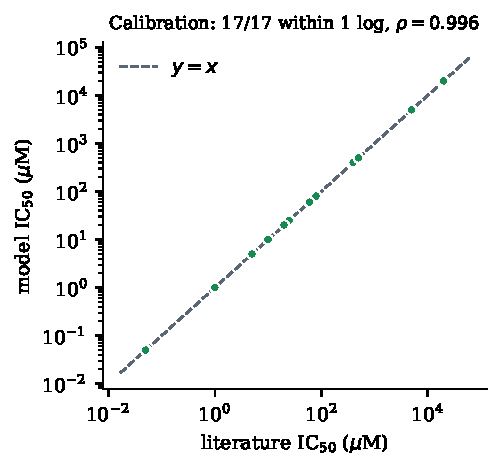
\includegraphics[width=0.82\linewidth]{figures/fig_calibration.pdf}
\caption{Model versus literature cytotoxic IC$_{50}$ for eighteen reference
toxins (log--log). All toxins fall within one order of magnitude of the anchor
and the cross-compound ordering is preserved.}
\label{fig:calibration}
\end{figure}

\subsection{Bayesian IC$_{50}$ with Credible Intervals}

Fig.~\ref{fig:bayes} shows HMC calibration for rotenone: the posterior median
dose--response with a $90\%$ credible band, and the resulting IC$_{50}$ posterior
$16.8\,\mu$M ($90\%$ CI $15.8$--$18.1$). The sampler mixed well
($\hat R=0.999$), and the identifiability shrinkage was $0.94$
(``well constrained by data''). In a recovery experiment where synthetic data
were generated at a known potency multiplier of $0.7$, the posterior recovered
$0.67$, confirming the pipeline is correctly calibrated.

\begin{figure}[!t]
\centering
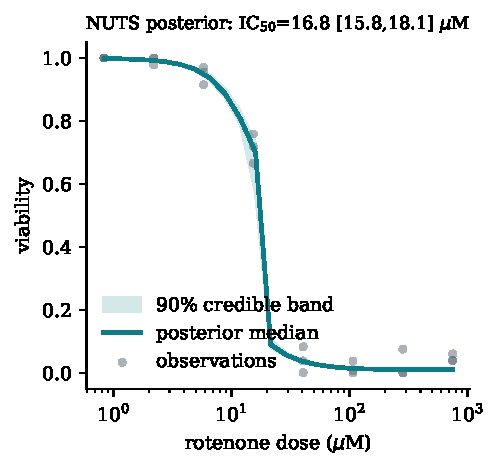
\includegraphics[width=0.82\linewidth]{figures/fig_bayes.pdf}
\caption{Bayesian (NUTS) calibration of rotenone: posterior-median dose--response,
$90\%$ credible band, and the observations used. The mechanistic ODE is the
forward model; gradients propagate through a differentiable re-implementation.}
\label{fig:bayes}
\end{figure}

\subsection{Online Data Assimilation}

Fig.~\ref{fig:assim} shows the particle filter recovering an unknown
electron-transport inhibition severity from a noisy time course of ATP and ROS.
The posterior mean converges to the true value ($0.70$; recovered
$0.70$) and, crucially, the $90\%$ credible band contracts from width
$0.15$ early to $0.06$ by the final observation---the twin becomes more
certain as evidence accumulates, the operational meaning of
Theorem~\ref{thm:contraction}.

\begin{figure}[!t]
\centering
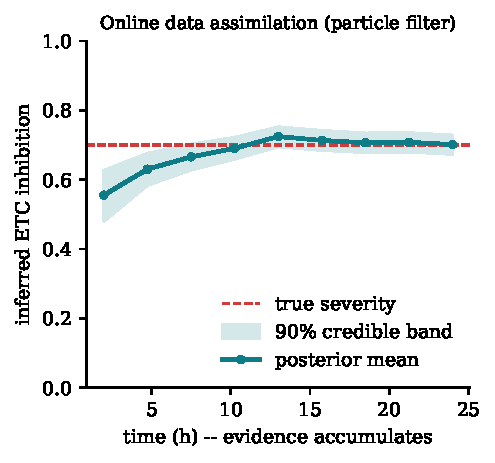
\includegraphics[width=0.82\linewidth]{figures/fig_assimilation.pdf}
\caption{Online assimilation of an unknown exposure severity by a particle
filter. The credible band contracts as measurements arrive.}
\label{fig:assim}
\end{figure}

\subsection{Tissue Selectivity Across Cell Types}

The same toxin acts differently on different cell types, which the twin captures
through cell-type-specific physiology (energy dependence, antioxidant reserve,
repair, apoptotic propensity, and CYP capacity). Fig.~\ref{fig:selectivity}
compares IC$_{50}$ across five cell types for three toxins: the model reproduces
anthracycline (doxorubicin) sensitivity of cardiomyocytes over hepatocytes,
cisplatin selectivity for the renal proximal tubule, and broad resistance of the
tumor line. The twin also reproduces qualitatively known behavior not shown here:
acetaminophen and carbon tetrachloride are toxic only where CYP bioactivation is
present, and glutathione-synthesis blockade sensitizes cells to oxidants
(buthionine sulfoximine synergizes with H$_2$O$_2$).

\begin{figure}[!t]
\centering
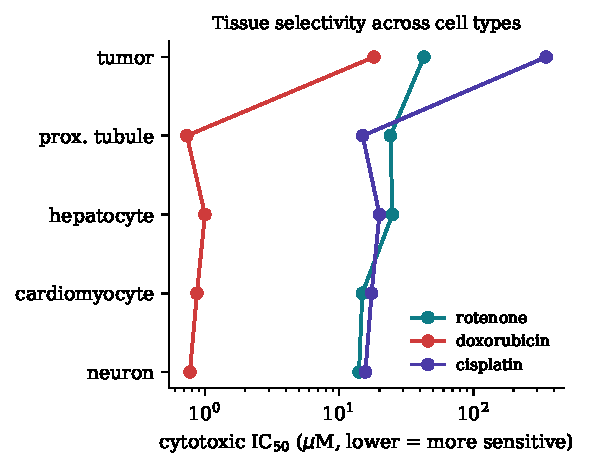
\includegraphics[width=0.82\linewidth]{figures/fig_selectivity.pdf}
\caption{Cytotoxic IC$_{50}$ of three toxins across five cell types. Lower is
more sensitive; the model reproduces known tissue selectivity.}
\label{fig:selectivity}
\end{figure}

\subsection{Population Heterogeneity and a Fast Surrogate}

A single deterministic cell dies switch-like; real tissue is a population of
cells with heterogeneous sensitivity. Modeling per-cell sensitivity as a
log-normal multiplier turns the steep single-cell response into the smooth
population sigmoid a real assay measures (Fig.~\ref{fig:population}). Finally, to
support high-throughput screening we train a multilayer-perceptron surrogate that
emulates the ODE endpoints from the modifier vector; it attains test
$R^2=0.93$ overall and $R^2\ge0.96$ on the graded endpoints (ATP, GSH,
membrane), with the switch-like death readouts less accurately emulated---an
honest limitation of emulating a threshold with a smooth network.

\begin{figure}[!t]
\centering
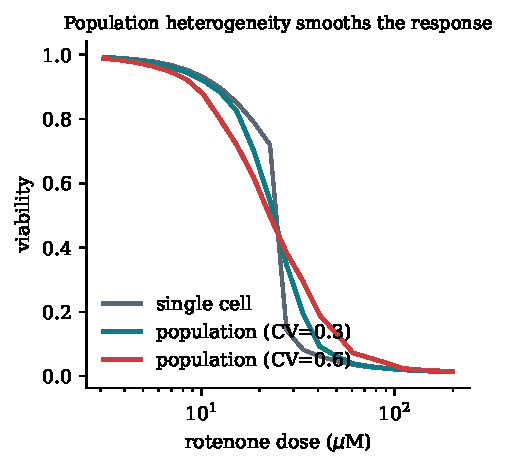
\includegraphics[width=0.82\linewidth]{figures/fig_population.pdf}
\caption{Cell-population heterogeneity smooths the switch-like single-cell
dose--response into the graded sigmoid measured in practice, with steepness
decreasing as biological variability (CV) increases.}
\label{fig:population}
\end{figure}

\subsection{Digital Twin Predictive Trajectories}

Fig.~\ref{fig:twin} shows the twin propagating posterior parameter uncertainty
through \eqref{eq:atp}--\eqref{eq:damage} at a fixed rotenone exposure, giving a
$90\%$ predictive band for every state. Consistent with
Theorem~\ref{thm:wellposed}, every sampled trajectory---and hence the entire
band---remains within the admissible ranges $\mathrm{ATP},\mathrm{ROS},\mathrm{GSH}\ge0$
and $\mathrm{CASP},\mathrm{MEM}\in[0,1]$.

\begin{figure}[!t]
\centering
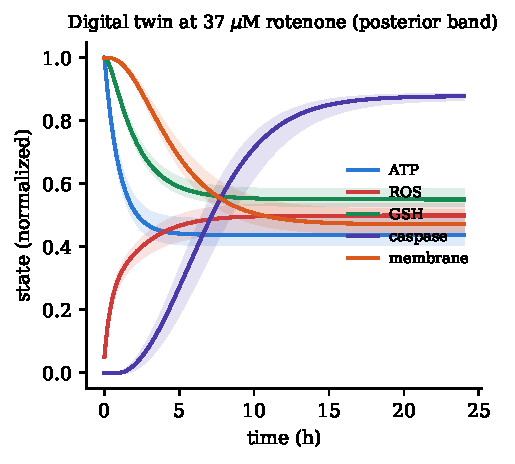
\includegraphics[width=0.82\linewidth]{figures/fig_twin.pdf}
\caption{Digital-twin predictive trajectories of the five state variables under a
fixed rotenone exposure; shaded bands are $90\%$ posterior predictive envelopes.}
\label{fig:twin}
\end{figure}

\section{Discussion}
\label{sec:discussion}

Several limitations bound these claims. First, calibration targets are
representative literature anchors, not a blind held-out set; the strongest test of
predictive accuracy---calibrating on a subset and predicting withheld compounds or
time courses from independent assays---remains future work, and the present
agreement should be read as internal consistency plus correct ordering rather than
external prediction. Second, the theoretical results we invoke are individually
classical; their value here is instantiation and validation on a concrete,
certified, open twin, not mathematical novelty. Third, the model is a single
well-mixed cell with normalized, dimensionless states; absolute concentrations,
spatial structure, and inter-cellular signaling are abstracted away. Fourth,
adaptive design is analyzed myopically; non-myopic campaign design requires
dynamic programming over $\mathcal{U}$ and is not treated. Finally, as with any
mechanistic model, $\theta^\star$ is the best-fitting parameter under the assumed
structure rather than a literal physiological ground truth; the identifiability
diagnostic is intended to keep this honest.

\section{Conclusion}
\label{sec:conclusion}

We presented a cell digital twin for in-silico toxicology that is globally well
posed on the biologically admissible domain, calibrated within Bayesian
uncertainty by Hamiltonian Monte Carlo through a differentiable re-implementation
of its dynamics, and updated online by a particle filter. Validated against
literature cytotoxicity for eighteen toxins across five cell types, it places all
toxins within one order of magnitude, reproduces cross-compound potency ordering
and known tissue selectivity, and yields calibrated IC$_{50}$ credible intervals
with an explicit identifiability diagnostic. By combining a certified mechanistic
core with modern uncertainty quantification and data assimilation in an open,
reproducible package, the twin is positioned as a transparent instrument for
mechanism-aware, uncertainty-driven toxicity screening.

\begin{thebibliography}{30}
\bibitem{bloomingdale2017} P.~Bloomingdale \emph{et~al.}, ``Quantitative systems toxicology,'' \emph{Curr. Opin. Toxicol.}, vol.~4, pp.~79--87, 2017.
\bibitem{watkins2020} P.~B.~Watkins, ``DILIsym: Quantitative systems toxicology impacting drug development,'' \emph{Curr. Opin. Toxicol.}, vol.~23--24, pp.~67--73, 2020.
\bibitem{yang2022} H.~Yang \emph{et~al.}, ``Mechanistic modeling of drug-induced cellular toxicity,'' \emph{CPT Pharmacometrics Syst. Pharmacol.}, vol.~11, pp.~1--15, 2022.
\bibitem{albeck2008} J.~G.~Albeck \emph{et~al.}, ``Modeling a snap-action, variable-delay switch controlling extrinsic cell death,'' \emph{PLoS Biol.}, vol.~6, no.~12, e299, 2008.
\bibitem{laubenbacher2022} R.~Laubenbacher \emph{et~al.}, ``Digital twins in medicine,'' \emph{Nat. Comput. Sci.}, vol.~2, pp.~757--760, 2022.
\bibitem{corral2020} K.~Corral-Acero \emph{et~al.}, ``The `digital twin' to enable the vision of precision cardiology,'' \emph{Eur. Heart J.}, vol.~41, no.~48, pp.~4556--4564, 2020.
\bibitem{gutenkunst2007} R.~N.~Gutenkunst \emph{et~al.}, ``Universally sloppy parameter sensitivities in systems biology models,'' \emph{PLoS Comput. Biol.}, vol.~3, no.~10, e189, 2007.
\bibitem{transtrum2015} M.~K.~Transtrum \emph{et~al.}, ``Perspective: Sloppiness and emergent theories,'' \emph{J. Chem. Phys.}, vol.~143, no.~1, 010901, 2015.
\bibitem{blanchini1999} F.~Blanchini, ``Set invariance in control,'' \emph{Automatica}, vol.~35, no.~11, pp.~1747--1767, 1999.
\bibitem{khalil2002} H.~K.~Khalil, \emph{Nonlinear Systems}, 3rd ed. Prentice Hall, 2002.
\bibitem{sarkka2013} S.~S\"arkk\"a, \emph{Bayesian Filtering and Smoothing}. Cambridge Univ. Press, 2013.
\bibitem{rao1945} C.~R.~Rao, ``Information and accuracy attainable in the estimation of statistical parameters,'' \emph{Bull. Calcutta Math. Soc.}, vol.~37, pp.~81--91, 1945.
\bibitem{vandervaart1998} A.~W.~van~der~Vaart, \emph{Asymptotic Statistics}. Cambridge Univ. Press, 1998.
\bibitem{hoffman2014} M.~D.~Hoffman and A.~Gelman, ``The No-U-Turn sampler,'' \emph{J. Mach. Learn. Res.}, vol.~15, pp.~1593--1623, 2014.
\bibitem{phan2019} D.~Phan, N.~Pradhan, and M.~Jankowiak, ``Composable effects for flexible and accelerated probabilistic programming in NumPyro,'' \emph{arXiv:1912.11554}, 2019.
\bibitem{cover2006} T.~M.~Cover and J.~A.~Thomas, \emph{Elements of Information Theory}, 2nd ed. Wiley, 2006.
\bibitem{lindley1956} D.~V.~Lindley, ``On a measure of the information provided by an experiment,'' \emph{Ann. Math. Statist.}, vol.~27, no.~4, pp.~986--1005, 1956.
\bibitem{chaloner1995} K.~Chaloner and I.~Verdinelli, ``Bayesian experimental design: A review,'' \emph{Statist. Sci.}, vol.~10, no.~3, pp.~273--304, 1995.
\bibitem{bhatia1997} R.~Bhatia, \emph{Matrix Analysis}. Springer, 1997.
\bibitem{gordon1993} N.~J.~Gordon, D.~J.~Salmond, and A.~F.~M.~Smith, ``Novel approach to nonlinear/non-Gaussian Bayesian state estimation,'' \emph{IEE Proc. F}, vol.~140, no.~2, pp.~107--113, 1993.
\bibitem{doucet2001} A.~Doucet, N.~de~Freitas, and N.~Gordon, Eds., \emph{Sequential Monte Carlo Methods in Practice}. Springer, 2001.
\bibitem{karr2012} J.~R.~Karr \emph{et~al.}, ``A whole-cell computational model predicts phenotype from genotype,'' \emph{Cell}, vol.~150, no.~2, pp.~389--401, 2012.
\bibitem{virtanen2020} P.~Virtanen \emph{et~al.}, ``SciPy 1.0: fundamental algorithms for scientific computing in Python,'' \emph{Nat. Methods}, vol.~17, pp.~261--272, 2020.
\end{thebibliography}

\end{document}
